% \documentclass{article}
\documentclass[../../outputs/main.tex]{subfiles}

% Any packages or configurations specific to this section
\usepackage{lipsum}
\usepackage{graphicx}

\begin{document}

\section{Case Study Demonstration}
% The energy price data is taken from the ComEd hourly live prices data \cite{comedLivePrices} for 10 November 2023. 

\subsection{Simulation Data: IEEE 123 Bus Test System}
The case studies are conducted on the balanced three-phase version of the IEEE 123 bus test system, which has $85$ Load Nodes. Additionally, $20 \% \, (17)$ and $30 \% \, (26)$ of these load nodes also contain reactive power controllable PVs and BESS, respectively. Their ratings are as per \Cref{table:parameter-values}. To demonstrate the effectiveness of the proposed algorithm, the test system is divided into four areas as shown in \Cref{fig:ieee123-four-area-figure}. It is assumed that a horizon-wide forecast for loads $p^t_L$, solar power output $p^t_D$ and cost of substation power  $C^t$ is available to the distribution system operator. Initially, the study is carried out for 5 hours with input data shown in \Cref{fig:inputCurve-5}. The five-hour workflow is described below. 

\def\ds{\rule{0pt}{1.5ex}} % this will lower the subscript by that amount, useful for $p_{D_{R_j}}$ where otherwise p and D appear to be almost at the same level.

\begin{table}[t]
    \centering
    \caption{Parameter values}
    \begin{tabular}{|l|c|}
    \hline
    \textbf{Parameter} & \textbf{Value} \\ \hline
    $V_{min}, V_{max}$ & 0.95\, pu, 1.05\, pu \\ \hline
    $p_{\ds D_{R_j}}$ & $0.33 p_{\ds L_{R_j}}$ \\ \hline
    $S_{D_{R_j}}$ & $1.2 p_{\ds D_{R_j}}$ \\ \hline
    $P_{B_{R_j}}$ & $0.33 p_{\ds L_{R_j}}$ \\ \hline
    $S_{B_{R_j}}$ & $1.2 P_{\ds B_{R_j}}$ \\ \hline
    $B_{R_j}$ & $T_{fullCharge} \times P_{B_{R_j}}$ \\ \hline
    $T_{fullCharge}$ & 4 h \\ \hline
    $\Delta t$ & 1 h \\ \hline
    $\eta_c, \eta_d$ & 0.95, 0.95 \\ \hline
    $soc_{min}, soc_{max}$ & 0.30, 0.95 \\ \hline
    $\alpha$ & 0.001 \\ \hline
    \end{tabular}
    \label{table:parameter-values}
\end{table}

\begin{figure}[t]
    \centering
    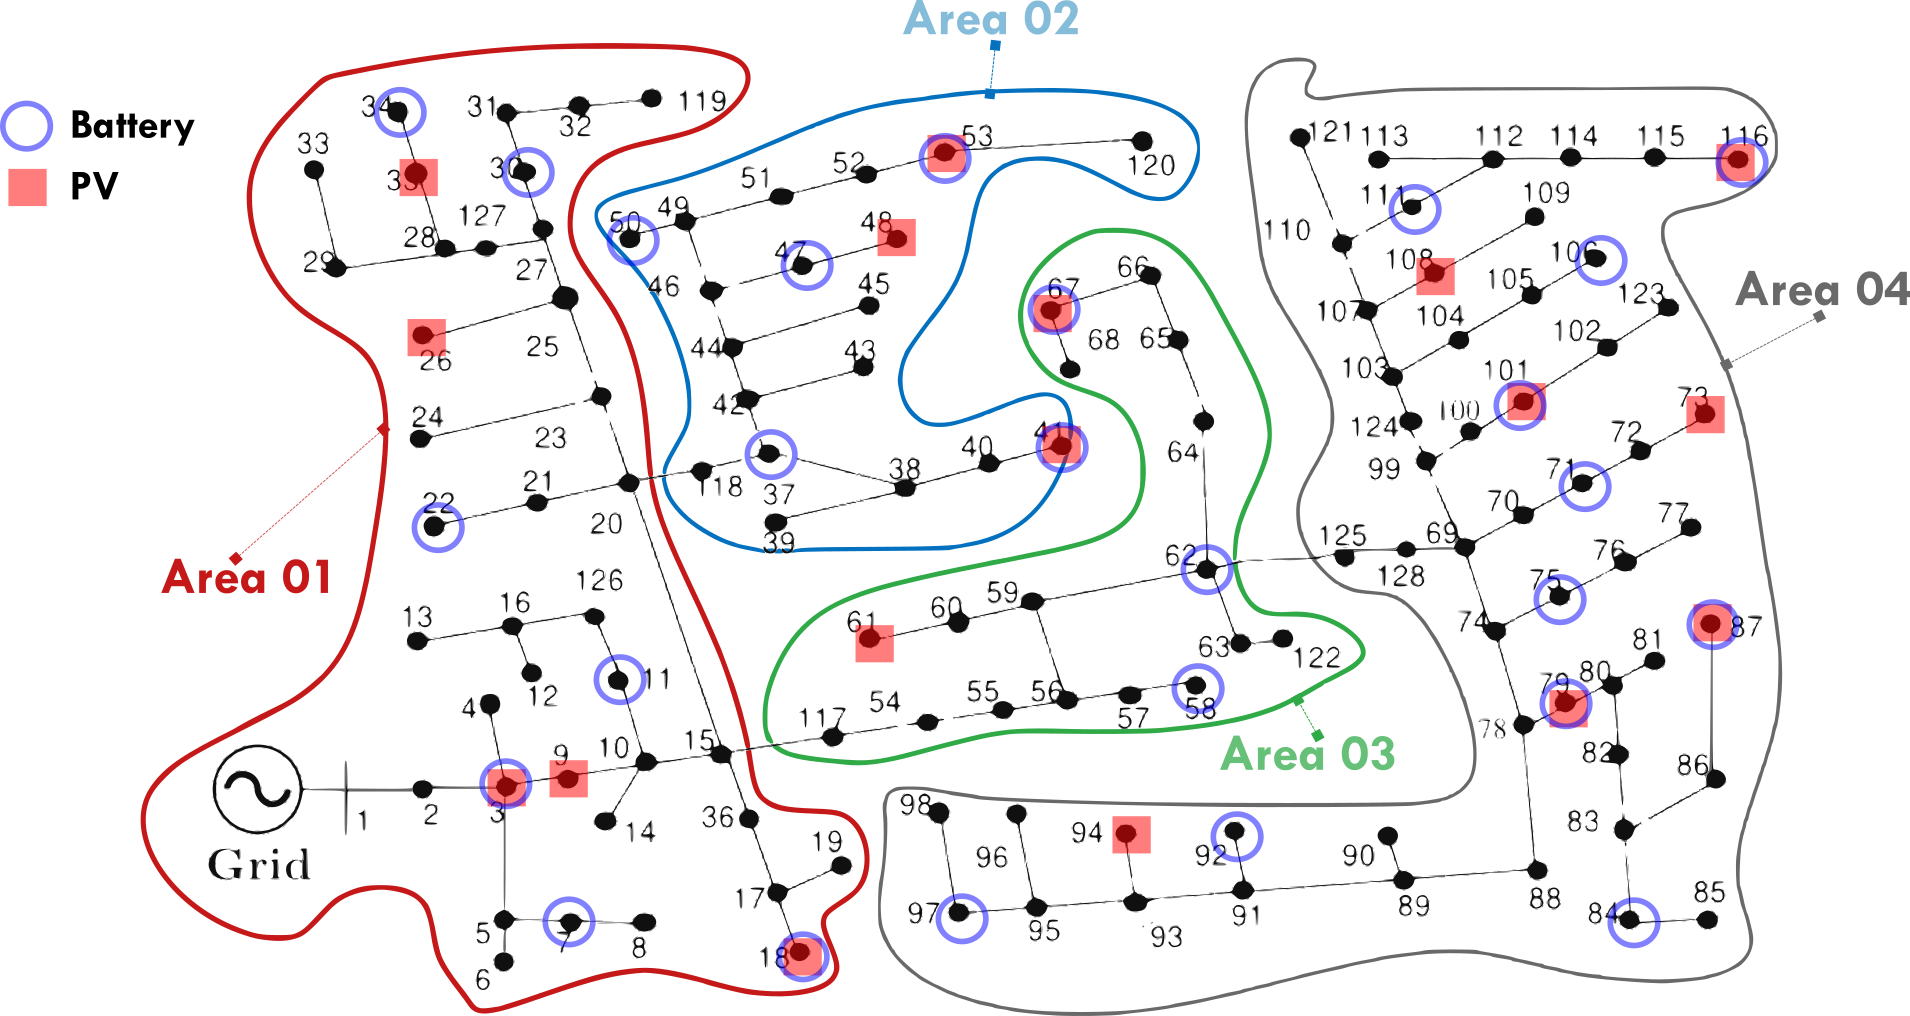
\includegraphics[width=\linewidth]{../figures/ieee123-FourAreas-pv20-batt30.png}
    \caption{IEEE 123 node system divided into four areas}
    \label{fig:ieee123-four-area-figure}
    \vspace{-4mm}
\end{figure}

% To showcase the workflow of the proposed algorithm, simulations were run for a $5$ time-period horizon. 

\begin{figure}[t]
    \centering
    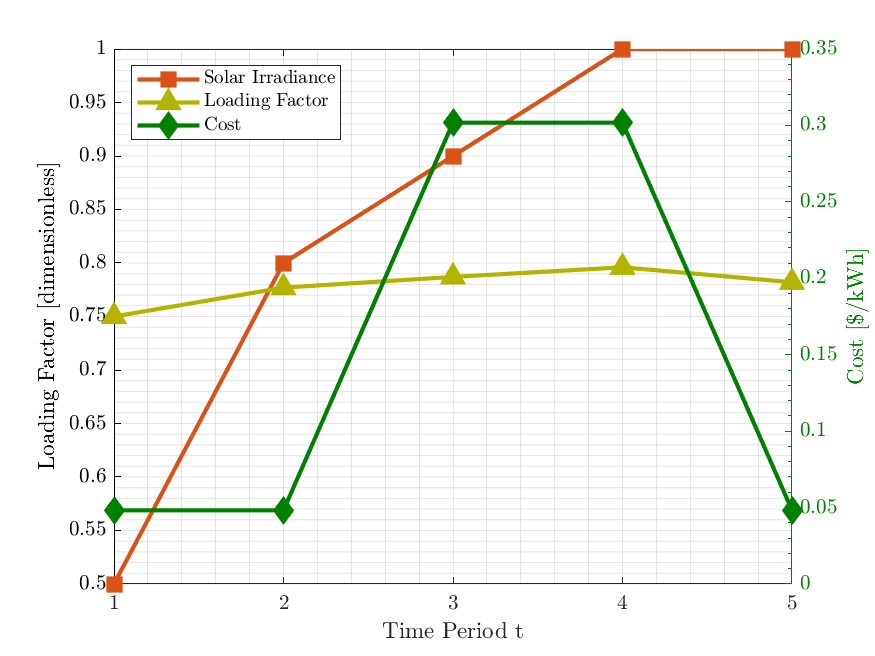
\includegraphics[height=0.25\textheight]{../figures/T5-inputCurves/InputCurves_Horizon_5.png}
    \caption{Forecasts for demand power, irradiance and cost of substation power over a 5 hour horizon}
    \label{fig:inputCurve-5}
    \vspace{-4mm}
\end{figure}

\def\ds{\rule{0pt}{1.5ex}} % this will lower the subscript by that amount, useful for $p_{D_{R_j}}$ where otherwise p and D appear to be almost at the same level.



\subsection{Simulation Workflow}

All simulations were set up in MATLAB 2023a including both the high level algorithms as well as calls to the optimization solver. MATLAB's \texttt{fmincon} function was used to parse the nonlinear nonconvex optimization problem described by \crefrange{eq:genCost_withSCD}{eq:modelEndsHere-and-lim_Bj} in tandem with the SQP optimization algorithm to solve it. From the completed simulations, the resultant optimal control variables were obtained, and were passed through an OpenDSS engine (already configured with system data and forecast values) in order to check for the ACOPF feasibility of the results. 
% The associated code may be found \href{https://github.com/Realife-Brahmin/MultiPeriod-DistOPF-Benchmark}{here}. 
The associated code may be found in \cite{MPOPFRepo}. 
As the IEEE 123 bus system is decomposed into 4 areas, so the total number of variables exchanged at each iteration for the 5-hour simulation of the MPDOPF is \(2*3*5=30\).

% \href{https://t.ly/dUCfC}{here}. % shortened link

\end{document}
